\section{Software Frameworks and Application Frameworks}
A software Framework is a collection of \emph{common code} providing \emph{generic functionalities} that can be \emph{selectively overridden or specialized} by user code providing \emph{specific functionality}.

An application framework is a software framework used to implement the \emph{standard} structure of an application for a \emph{specific} development environment.

Some categories of software frameworks are:
\begin{itemize}
    \item GUI frameworks:
    \begin{itemize}
        \item MFC: Microsoft Foundation Class Library is a C++ object-oriented library for windows;
        \item Gnome: written in C, mainly for Linux;
        \item Qt: it's a cross platform GUI framework written in C++.
    \end{itemize}
    \item web frameworks (based on Model-View-Controller design pattern):
    \begin{itemize}
        \item ASP.NET: C\# framework made from Microsoft for web sites, web applications and web services;
        \item GWT: Google Web Toolkit;
        \item Rails: written in Ruby, provides default structures for databases, web services and web pages;
        \item Spring: Java-based enterprise web applications;
        \item Flask: micro-framework in python, highly extensible with the various modules;
        \item Django: python comprehensive web framework.
    \end{itemize}
    \item concurrency frameworks:
    \begin{itemize}
        \item Hadoop Map/Reduce: software framework for applications which process big amounts of data in parallel on large clusters in a fault-tolerant manner.
        The Map functionality takes input data and converts it into a set of tuples (key/value pairs) while the Reduce functionality takes the output from Map and combines the data tuples into a smaller set of tuples.
    \end{itemize}
\end{itemize}

Some known general software frameworks are:
\begin{itemize}
    \item .NET;
    \item Android SDK: supports development of apps in Java not using the JVM (it uses the dalvik);
    \item Cocoa: Apple's native OO API for MacOS which includes C standard library and the Objective-C runtime;
    \item Eclipse: cross-platform, extensible IDE with plugins.
\end{itemize}

\subsection{Component Framework}
A component framework is a framework that supports development, deployment, composition and execution of components designed according to a given \emph{Component Model}.
The support for the development of components enforces the design of precise interfaces and the support for the composition and connection follows the mechanisms provided by the component model.

Of course those framework provides already prebuilt functionalities such as useful components or automated assembly functions that automatically instantiate and compose components to perform common tasks.
The component framework establishes environmental conditions for the component instances ad regulates the interaction between component instances.

\section{Features of Frameworks}
A framework embodies some abstract design, with more behavior built in.
In order to use it you need to insert your behavior into various places in the framework either by subclassing or by plugging in your own classes then the framework's code calls your code when needed.

The very general concept is \emph{inversion of control}: rather than your code calling the library code is the framework that calls your code, this is the main difference between libraries and frameworks.

A framework is mainly made by:
\begin{itemize}
    \item libraries with APIs;
    \item ready-made extensible programs (called engines);
    \item sometimes also tools for development, configuration, etc.
\end{itemize}

\subsection{Extensibility}
All frameworks can be extended to cater for application specific functionality because it is the intended way of using one.
Common ways to extend a framework are:
\begin{itemize}
    \item extension within the framework language: by subclassing and overriding methods, by implementing interfaces and registering event handlers;
    \item plug-ins: let the framework loads certain extra code in a specific format.
\end{itemize}

\section{Inversion of Control}

\subsection{In GUI}
In a text-based interaction, the order of interactions and of invocations is decided by the code while in a GUI-based interaction the developer specifies the layout and binds the event-listener to the component, then is the GUI loop that decides when to invoke those methods, based on the order of events.

\subsection{In General}
\begin{figure}[H]
    \centering
    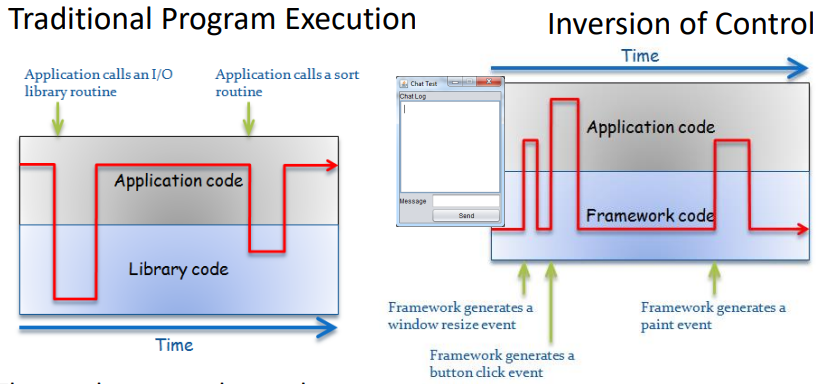
\includegraphics[width=300px]{images/9_Frameworks/IOC.png}
    \caption{Library vs framework}
\end{figure}

Sometimes the keyword framework is used in order to intend "well-designed library" like in Java Collection Framework, but it's not so correct.

Control is not only intended as control flow but also control over dependencies, coupling and configuration.
The dependency injection is a way to enable inversion of control respect to dependencies because something outside a component handles the configuration and wiring of the dependencies, moreover it removes coupling of configuration to the point of use and coupling of component to concrete dependent components.
It's in some sense contrary to encapsulation.

\subsection{Containers}
Often frameworks provide containers for deploying components which may provide functionalities needed by the components to execute.
For example EJB containers are responsible of the persistent storage of data and of the availability of EJB's for all authorized clients.

\section{Loosely coupled systems}
Good object oriented systems should be organised as network of interacting objects, the goal is to achieve high cohesion and low coupling because that increases:
\begin{itemize}
    \item extensibility;
    \item testability;
    \item reusability.
\end{itemize}

Let's take as an example a Trade Monitor application: a trader wants that the system rejects trades when the exposure reaches a certain limit, so the component TradeMonitor (that is a class in our example) provides a method \verb|TryTrade| which checks the condition.
The \emph{current exposure} and the \emph{exposure limit} are stored in some persistent storage and are accessed by the method itself through another component called \verb|DAO| (Data Access Object).
Let's see how we can implement this scenario: the first naive scenario is represented by the following diagram:
\begin{figure}[H]
    \centering
    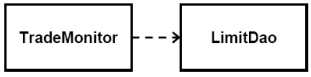
\includegraphics[width=200px]{images/9_Frameworks/trade_monitor_0.png}
    \caption{Trade Monitor version 0}
\end{figure}
we declare and build the \verb|LimitDao| inside the \verb|TradeMonitor| constructor.
This solution leads to tightly coupling between the two components and poses some problems:
\begin{itemize}
    \item extensibility: what if we replace the database with a distributed cache?
    \item testability: where do the limit for test come from?
\end{itemize}

We can then refactor introducing an interface \verb|LimitRepository| which implements the methods \verb|GetExposure| and \verb|GetLimit|, we can then create two implementations, one which uses the persistent storage and another one with test values.
This approach solves nothing because the constructor still has a static dependency on DAO object, independently by the implementation we decide to use.

A new version could use a \verb|Factory|, a class whose responsibility is to build the correct LimitDao implementation and return it to TradeMonitor once asked:
\begin{figure}[H]
    \centering
    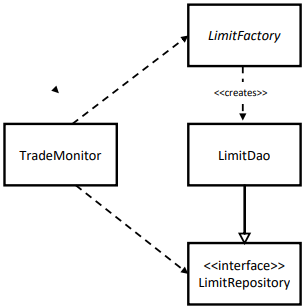
\includegraphics[width=200px]{images/9_Frameworks/trade_monitor_1.png}
    \caption{Trade Monitor version 1}
\end{figure}
This solution provides decoupling from LimitDao but now LimitDao is tightly-coupled with Factory.

\subsection{Service locator}
A Service Locator is an object that acts as a (static) registry for the LimitDao that the application needs.
An external unit sets up this global registry and then the TradeMonitor uses the Service Locator functionality to get the needed LimitDao implementation.
\begin{figure}[H]
    \centering
    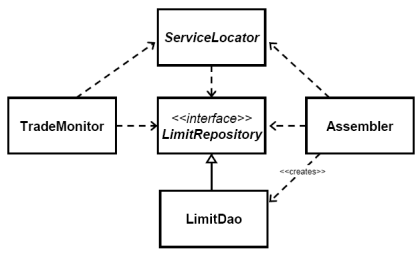
\includegraphics[width=250px]{images/9_Frameworks/trade_monitor_service_locator.png}
    \caption{Trade Monitor with Service Locator}
\end{figure}

The Service Locator patterns succeeds in decoupling the TradeMonitor from the LimitDao and allows new components to be dynamically created and used by other components later.
This pattern has though some drawbacks:
\begin{itemize}
    \item every components that needs a dependency must have a reference to the service locator;
    \item all components need to be registered with the service locator and the registration can be done:
    \begin{itemize}
        \item by name: which means that services can't be type checked, the component has a dependency to the dependent component name and if many components share an instance but later you want to specify different instance for some, some refactoring is needed;

        \item by type: which means that can only bind one instance of a type inside a container.
    \end{itemize}
    \item code needs to handle lookup problems (maybe using errors, default depedency, or other)
\end{itemize}

\subsection{Dependency injection}
Using this pattern the plugin is created by an external assembler and it is passed to TradeMonitor in some way, thus the dependency is not anymore in the code of the main component but it is injected into it.
Dependency injection allows avoiding hard-coded dependencies, so avoiding strong coupling, and changing them.
It can be done in different ways.
\begin{figure}[H]
    \centering
    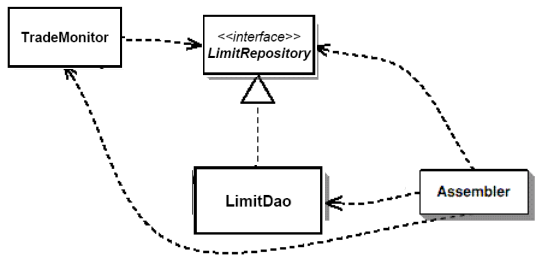
\includegraphics[width=250px]{images/9_Frameworks/trade_monitor_dependency_injection.png}
    \caption{Trade Monitor with Dependency Injection}
\end{figure}

\subsubsection{Setter injection}
The idea is to add a setter method to attach a dependency, leaving the creation and resolution to others.
It is widely used in Spring because it leverages existing JavaBean reflective pattern.
It is simple and often already available.
Though it makes possible to create partially constructed objects and advertises that dependency can be changed at runtime (as opposed to constructor).

\subsubsection{Constructors}
The idea is to add the dependency inside the constructor call, this solves the problem of partially constructed objects, it' simple and often already available.
Though it makes bidirectional dependencies between objects tricky, constructors can easily get big and parameters confusing, if a lot of optional dependencies are used it may leads to a lot of constructors and it makes the class evolution more complicated because various constructor must be touched.
Those last problems though can be solved using the Builder design patterns.

\section{Software Framework design}
The design of a software framework is an intellectual challenging task which requires a deep understanding of the application domain, mastering software design patterns, object oriented methods and polymorphism.

The understanding of frameworks is done in 4 areas:
\begin{itemize}
    \item understanding the applicable language concepts, like the one we've already said: inheritance, polymorphism, encapsulation and delegation;
    \item understanding the framework concepts and techniques sufficiently enough to use the framework in order to build custom applications;
    \item being able to do detailed design and implementation of frameworks for which the common and variable aspects are already known;
    \item learning to analyze a potential software family, identifying its possible common and variable aspects, and evaluating alternative framework architectures.
\end{itemize}

\subsection{A framework for the divide and conquer algorithms family}
Let's design, for example, a framework that can be used to implement divide and conquer algorithms.
We could provide the following core code:
\begin{verbatim}
    function solve (Problem p) returns Solution{
        if isSimple(p)
            return simplySolve(p);

        sp[] = decompose(p);
        for (i= 0; i < sp.length; i = i+1)
            sol[i] = solve(sp[i]);
        return combine(sol);
    }
\end{verbatim}
then we just need to create generic views for the methods used in this core and the user will need to create it's own instances and implementation for the single components while the framework will do the actual algorithm logic.

\subsection{Some terminology}
\begin{itemize}
    \item \emph{Frozen Spot}: common (shared) aspect of the software family;
    \item \emph{Hot Spot}: variable aspect of the family;
    \item \emph{hook methods}: abstract methods that represents hot spots;
    \item \emph{Template Method}: concrete method of base (abstract) class implementing behavior common to all members of the family. Those methods calls a hook method to invoke a function that is specific to one family member implementing inversion of control;
\end{itemize}
A hot spot is realized in a framework as a hot spot subsystem which is composed by an abstract base class and some concrete subclasses:
\begin{figure}[H]
    \centering
    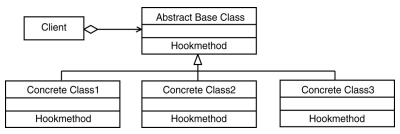
\includegraphics[width=300px]{images/9_Frameworks/hot_spot_subsystem.png}
    \caption{Hot Spot subsystem}
\end{figure}

\subsection{Framework construction}
To build a framework we can use one of those two principles:
\begin{itemize}
    \item \emph{unification principle} via the \emph{Template Method} design pattern: it uses inheritance to implement the hot spot subsystem, both the template methods and hook methods are defined in the same abstract base class and the hook methods are implemented in subclasses of the base class;

    \item \emph{separation principle} via the \emph{Strategy} design pattern: it uses delegation to implement the hot spot subsystem in which the template methods are implemented in a concrete context class, the hook methods are defined in a separate abstract class and implemented in its subclasses.
    The template methods delegate work to an instance of the subclass that implements the hook methods.
\end{itemize}
The two approaches differs in the coupling between client and chosen algorithm because in the case of strategy pattern the coupling is determined by dependency injection (using the strategy setter) and could change at runtime.


\subsubsection{Template Method}
It is one of the behavioural pattern described by the Gang of Four, it's intent is to define the skeleton of an algorithm in an operation, deferring some steps to subclasses.
A template methods belongs to an abstract class and it defines an algorithm in terms of abstract operations that subclasses override to provide concrete behavior.

Template methods call the following operations:
\begin{itemize}
    \item concrete operations of the abstract class (fixed parts of the algorithm);
    \item primitive operations: abstract operations that subclasses \emph{must} implement;
    \item hook operations: which provide default behavior that subclasses \emph{may} override if necessary.
    A hook operation often does nothing by default.
\end{itemize}

\begin{figure}[H]
    \centering
    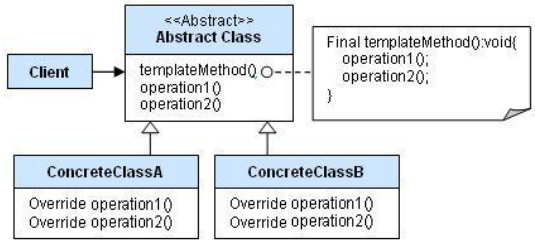
\includegraphics[width=300px]{images/9_Frameworks/template_method_UML.png}
    \caption{Template method UML}
\end{figure}

Some implementations could use:
\begin{itemize}
    \item in Java using visibility modifiers:
    \begin{itemize}
        \item the template method should not be overridden to it can be declared as public and final;
        \item the concrete operations can be declared as private ensuring that they are only called by the template methods;
        \item primitive operations that \emph{must} be overridden are declared as protected abstract;
        \item the hook operations that \emph{may} be overridden are declared as protected with a default implementation.
    \end{itemize}

    \item in C++ using access control:
    \begin{itemize}
        \item the template method itself should not be overridden so it can be declared as nonvirtual;
        \item the concrete operations can be declared as protected ensuring that they are only called by the template method;
        \item primitive operations that \emph{must} be overridden are declared as pure virtual;
        \item the hook operations that \emph{may} be overridden are declared as protected virtual.
    \end{itemize}
\end{itemize}

\subsubsection{Strategy}
It's one of the behavioral pattern described by the Gang of four and it's intent is to allow to select (part of) an algorithm at runtime.
The client uses an object implementing the interface and invokes methods of the interface for the hot spots of the algorithm.

\begin{figure}[H]
    \centering
    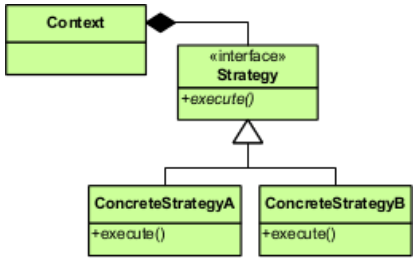
\includegraphics[width=250px]{images/9_Frameworks/strategy_UML.png}
    \caption{Strategy UML}
\end{figure}

\subsection{Framework development by generalization}
Framework design involves incrementally evolving a design rather than discovering it in one single step.
This evolution consists of:
\begin{itemize}
    \item examining existing designs for family members;
    \item identifying the frozen spots and hot spots of the family;
    \item generalizing the program structure to enable reuse of the code for frozen spots and use of different implementations for each hot spot.
\end{itemize}







